% ============================================================
% Chapter 5 --- Continuity
% Originally: content/week-02.tex, \section{Continuity} (Corsin Week 2, Friday)
%           + content/week-03.tex, the Lipschitz block that sat inside
%             \subsection{Why do we care about compactness?} (Corsin Week 3, Monday)
% ============================================================
\chapter{Continuity}
\label{ch:continuity}

% Transition: Claude Opus 5 (High)
% Lipschitz continuity is drawn from a second tutor's slides. It reached Corsin's own notes only
% obliquely, as a constant used for contraction mappings; sec:lipschitz_continuity names it
% properly and places it in the hierarchy.
With distance, shape and convergence in place, we can finally ask the question the whole
apparatus was built for. What does it mean for a map \emph{between} two metric spaces to respect
that structure?

Three answers are given, and they are equivalent: the $\varepsilon$--$\delta$ condition inherited
from \emph{Analysis I}, a sequential condition, and a topological one asking that preimages of
open sets be open. Having all three is not redundance. The first is what one verifies for a
concrete function, the second is what combines with the sequential arguments of the previous
chapter, and the third is the only one that survives when the metric is taken away. The chapter
then adds the two strengthenings needed later, uniform continuity and Lipschitz continuity, and
locates them in a hierarchy of increasingly demanding conditions.

% Originally: content/week-02.tex, \section{Continuity} (Corsin Week 2, Friday)

% Source: Corsin Nick/Class Notes/Week 2.pdf, pp. 1--13
\section{Continuity}
\label{sec:continuity}

\begin{definition}[Continuous map]
\label{def:continuous}
For $(X, d_X)$ and $(Y, d_Y)$ metric spaces, a function $f : X \to Y$ is called \newterm{continuous}
\germanfor{stetig} if one of the following equivalent conditions holds:
\begin{enumerate}[label=\textbf{(\alph*)}]
  \item \textbf{($\varepsilon$--$\delta$):} $\forall x_0 \in X, \varepsilon > 0 \ \exists \delta > 0$ such that for all $x \in X$:
    \[d(x_0, x) < \delta \implies d(f(x_0), f(x)) < \varepsilon\]
  \item \textbf{(Sequentially continuous):} for any sequence $(x_n)_{n=0}^{\infty}$ in $X$ with
    limit $x \in X$, $\lim_{n\to\infty} f(x_n) = f(x)$ (and the limit exists).
  \item \textbf{(Topological):} for all $U \subseteq Y$ open, $f^{-1}(U) \subseteq X$ is open
    (\cref{def:open_closed}).
\end{enumerate}
\end{definition}

\begin{ainote}
Corsin writes $d(x_0,x) < \varepsilon$ in the ($\varepsilon$--$\delta$) hypothesis above, which
must read $\delta$, since otherwise the quantified $\delta$ is never used at all. This is a slip
of the pen, and it is corrected in \cref{def:continuous}.
\end{ainote}

% Generator: Claude Opus 5 (High) --- \cref{def:continuous} asserts the equivalence of three
% conditions without proving it; the cycle is short and uses only results already available.
\begin{proposition}[The three definitions of continuity agree]
\label{prop:continuity_equivalences}
The conditions \textbf{(a)}, \textbf{(b)} and \textbf{(c)} of \cref{def:continuous} are
equivalent, so \cref{def:continuous} is well posed.
\end{proposition}

\begin{proof}
We prove the cycle
$\text{\textbf{(a)}} \Rightarrow \text{\textbf{(b)}} \Rightarrow \text{\textbf{(c)}}
\Rightarrow \text{\textbf{(a)}}$.

\textbf{(a) $\Rightarrow$ (b).} Let $x_n \to x$ and let $\varepsilon>0$. Pick $\delta>0$ as in
\textbf{(a)} for the point $x$, then $N$ with $d_X(x_n,x)<\delta$ for $n \geq N$. For those $n$,
$d_Y(f(x_n),f(x)) < \varepsilon$, so $f(x_n) \to f(x)$.

\textbf{(b) $\Rightarrow$ (c).} Let $U \subseteq Y$ be open and suppose $f^{-1}(U)$ were not.
By the shrinking-ball construction (\cref{rem:shrinking_ball_trick}) there are
$x \in f^{-1}(U)$ and points $x_n \in B_{1/n}(x)$ with $x_n \notin f^{-1}(U)$. Then $x_n \to x$,
so $f(x_n) \to f(x) \in U$ by \textbf{(b)}, and since $U$ is open,
\cref{prop:open_closed_via_sequences}\textbf{(a)} forces $f(x_n) \in U$ for large $n$. That is,
$x_n \in f^{-1}(U)$, which is a contradiction.

\textbf{(c) $\Rightarrow$ (a).} Fix $x_0 \in X$ and $\varepsilon>0$. The ball
$B_\varepsilon(f(x_0)) \subseteq Y$ is open (\cref{ex:ai_open_balls_are_open}), so
$f^{-1}\big(B_\varepsilon(f(x_0))\big)$ is open by \textbf{(c)} and contains $x_0$. Hence there
is $\delta>0$ with $B_\delta(x_0) \subseteq f^{-1}\big(B_\varepsilon(f(x_0))\big)$, which says
precisely that $d_X(x_0,x)<\delta$ implies $d_Y(f(x_0),f(x))<\varepsilon$.
\end{proof}

% Generator: Claude Opus 5 (High) --- FIG-05-01. The chapter defines continuity three ways and
% had no picture at all; its only figure was the Lipschitz cone, two sections later.
%
% GEOMETRY. Nothing here is a computation, so there is no arithmetic to check; what matters is
% that the drawing asserts only true things. Two deliberate choices:
%   * The image of B_delta(x_0) is drawn as an irregular blob strictly INSIDE B_epsilon(f(x_0)),
%     not as a disc and not filling it. Continuity says the image is contained in the target
%     ball; it says nothing about the image being round, being centred, or exhausting the ball.
%     A figure drawing f(B_delta) as a concentric disc would assert all three.
%   * The blob touches neither the boundary of B_epsilon nor f(x_0)'s dot, since the inclusion
%     is into the OPEN ball and f(x_0) is interior to the image, not on its edge.
% The same picture reads condition (c) backwards: B_delta sits inside the preimage of the open
% ball B_epsilon, which is the containment the proof of (c) => (a) produces.
\begin{center}
\begin{tikzpicture}[>=Latex, scale=1.0]
  % ---- the source space ----
  \draw[gray!55] plot[smooth cycle, tension=0.75] coordinates
    {(-2.5,1.15) (-0.85,1.5) (0.15,0.55) (-0.35,-1.2) (-1.9,-1.45) (-2.95,-0.25)};
  \node[gray!55!black, font=\small] at (-2.72,1.28) {$X$};
  \fill[MidnightBlue!8] (-1.45,0.05) circle (0.62);
  \draw[MidnightBlue!70, thick] (-1.45,0.05) circle (0.62);
  \fill[MidnightBlue!70] (-1.45,0.05) circle (1.4pt);
  \node[MidnightBlue!70, font=\scriptsize, anchor=north east] at (-1.5,-0.02) {$x_0$};
  \node[MidnightBlue!70, font=\scriptsize, anchor=south] at (-1.45,0.70) {$B_\delta(x_0)$};

  % ---- the map ----
  \draw[->, thick] (0.55,0.05) -- (1.95,0.05) node[midway, above, font=\small] {$f$};

  % ---- the target space ----
  \draw[gray!55] plot[smooth cycle, tension=0.75] coordinates
    {(2.6,1.3) (4.4,1.5) (5.5,0.4) (4.9,-1.3) (3.3,-1.5) (2.35,-0.3)};
  \node[gray!55!black, font=\small] at (5.35,1.15) {$Y$};
  \fill[BrickRed!7] (3.95,0.05) circle (0.78);
  \draw[BrickRed!80, thick] (3.95,0.05) circle (0.78);
  \node[BrickRed!80, font=\scriptsize, anchor=south] at (3.95,0.86)
    {$B_\varepsilon(f(x_0))$};

  % The image: irregular, strictly inside, not centred. All three are deliberate.
  \fill[OliveGreen!14] plot[smooth cycle, tension=0.8] coordinates
    {(3.72,0.42) (4.25,0.3) (4.38,-0.12) (3.95,-0.42) (3.55,-0.18)};
  \draw[OliveGreen, thick] plot[smooth cycle, tension=0.8] coordinates
    {(3.72,0.42) (4.25,0.3) (4.38,-0.12) (3.95,-0.42) (3.55,-0.18)};
  \fill[BrickRed!80] (3.95,0.02) circle (1.4pt);
  % Anchored below the dot and inside the blob. Anchored east it extended leftwards across the
  % blob's own outline at x = 3.55, so the label sat half in and half out of the region it names.
  \node[BrickRed!80, font=\scriptsize, anchor=north] at (3.95,-0.04) {$f(x_0)$};
  \node[OliveGreen, font=\scriptsize, anchor=north west] at (4.35,-0.35)
    {$f\big(B_\delta(x_0)\big)$};
\end{tikzpicture}
\end{center}

Condition \textbf{(a)} is the statement that the green region fits inside the red ball, and that
a $\delta$ making it fit can be found however small the red ball is made. Condition \textbf{(c)}
is the same picture read from right to left: $B_\delta(x_0)$ lies inside
$f^{-1}\big(B_\varepsilon(f(x_0))\big)$, which is exactly the containment produced in the
\textbf{(c)} $\Rightarrow$ \textbf{(a)} step above. Note what the drawing does not claim: the
image need not be round, need not be centred at $f(x_0)$, and need not fill the ball.

\begin{remark}[Which of the three to reach for]
Condition \textbf{(c)} is the only one that never mentions the metric. That is why it, and not the
$\varepsilon$--$\delta$ formulation, is what survives into general topology
(\cref{sec:structured_spaces}). Condition \textbf{(b)} is usually the fastest way to prove a
function is \emph{dis}continuous, since a single badly chosen sequence suffices; this is exactly
how \cref{ex:partial_derivatives_not_continuous} works. Condition \textbf{(a)} is the
one to use when a quantitative modulus is wanted, as in
\cref{def:uniformly_continuous} immediately below.
\end{remark}

% Sonnet 5 (Medium)
\begin{definition}[Uniform continuity]
\label{def:uniformly_continuous}
For $(X,d_X)$ and $(Y,d_Y)$ metric spaces, a function $f : X \to Y$ is \newterm{uniformly
continuous} \germanfor{gleichm\"assig stetig} if
\[\forall \varepsilon > 0 \ \exists \delta > 0 \ \forall x, x' \in X : \quad d_X(x,x') < \delta \ \text{ implies } \ d_Y(f(x),f(x')) < \varepsilon.\]
\end{definition}

\begin{importantremark}[Where the quantifiers sit]
\label{rem:continuity_vs_uniform_continuity}
Compare \cref{def:continuous} \textbf{(a)} with \cref{def:uniformly_continuous}: the
\emph{formulas} differ only in the order of two quantifiers, and that order is the whole
content.
\begin{itemize}
  \item \textbf{Continuity:} $\forall x_0\ \forall\varepsilon\ \exists\delta$. The point $x_0$
    is chosen \emph{before} $\delta$, so $\delta$ may depend on it, and a different $\delta$ is
    allowed at every point.
  \item \textbf{Uniform continuity:} $\forall\varepsilon\ \exists\delta\ \forall x$. Now
    $\delta$ is chosen \emph{before} seeing the point, so one and the same $\delta$ must work
    everywhere at once.
\end{itemize}
Uniform continuity is therefore strictly stronger. The standard witness is
$f(x) := 1/x$ on $(0,1)$: it is continuous, but near $0$ the graph steepens without bound, so
the $\delta$ that works at $x_0 = \tfrac12$ is hopeless at $x_0 = \tfrac{1}{1000}$, and no
single $\delta$ survives. \Cref{prop:compact_implies_uniformly_continuous} below says that on a
\emph{compact} space this can never happen. The gap between the two notions closes exactly when
there is no room left to run off towards a bad point.
\end{importantremark}

\begin{example}[$f(x) = x^2$]
Let $f : \mathbb{R} \to \mathbb{R}, x \mapsto x^2$. Let $a < b \in \mathbb{R}$. Then
\begin{itemize}
  \item for $a < 0 < b$: $\quad f^{-1}((a,b)) = (-\sqrt{b}, \sqrt{b})$, which is open.
  \item for $a < b < 0$: $\quad f^{-1}((a,b)) = \emptyset$.
  \item for $0 < a < b$: $\quad f^{-1}((a,b)) = (-\sqrt{b}, -\sqrt{a}) \cup (\sqrt{a}, \sqrt{b})$.
\end{itemize}
\textit{Why is it enough to check only these cases?} Hint:
$f^{-1}(U_1 \cup U_2) = f^{-1}(U_1) \cup f^{-1}(U_2)$.
\end{example}

% Source: Jérôme Paschoud/Notizen/Woche 4.1 Normen, das Differential.pdf, p. 2
% Generator: Gemini 3.1 Pro (High)
\begin{example}[Limits in $\mathbb{R}^2$ depend on the path]
\label{ex:limits_in_r2}
When computing limits in $\mathbb{R}^n$, one must ensure that the limit exists and is identical along \emph{all} possible paths approaching the point. For example, consider the function $f: \mathbb{R}^2 \setminus \{(0,0)\} \to \mathbb{R}$ given by $f(x,y) = \frac{x^2}{x^2+y^2}$.
If we approach the origin along the $x$-axis (setting $y=0$ first), we get
\[
\lim_{x \to 0} f(x, 0) = \lim_{x \to 0} \frac{x^2}{x^2} = 1.
\]
However, if we approach along the $y$-axis (setting $x=0$ first), we get
\[
\lim_{y \to 0} f(0, y) = \lim_{y \to 0} \frac{0}{y^2} = 0.
\]
Since these limits disagree, $\lim_{(x,y) \to (0,0)} f(x,y)$ does not exist. A robust method to check limits at the origin uniformly across all directions is to switch to \newterm{polar coordinates} ($x = r\cos\varphi, y = r\sin\varphi$). If the limit as $r \to 0$ is independent of $\varphi$, then the function converges. (This is explored further in \cref{ex:3.2}).
\end{example}

\begin{question}
Let $(X, d_X)$ and $(Y, d_Y)$ be metric spaces, where $d_Y$ is the discrete metric. Is
\emph{every} function $f : (X,d_X) \to (Y,d_Y)$ continuous?
\end{question}

\begin{answer}
\textbf{No.} For example, take the spaces $X = Y = \mathbb{R}$, $d_X$ the standard metric, and
$f = \id : X \to Y, z \mapsto z$. Then $\{0\} \subseteq Y$ is open, but
$\{0\} = \id^{-1}(\{0\})$ is not open in $(X, d_X)$.
\end{answer}

\begin{question}
And what if the roles are reversed, with $d_X$ the discrete metric and $d_Y$ arbitrary?
\end{question}

\begin{answer}
\textbf{Any} subset of $X$ is open; therefore, $f^{-1}(U)$ is open for any open $U \subseteq Y$. So
every such $f$ is continuous.
\end{answer}

% The old chapter continued from here into "Completeness"; that topic is now
% \cref{ch:completeness}, whose opening paragraph carries this transition.


% --- exercises relocated here from the dissolved sheets ---

% Originally: content/exercise-sheets/week-02.tex, problem 2.6
% Source: exercises/Ex2_Analysis2_eng.pdf, p. 1

\begin{exercise}[Continuity of the distance]
\label{ex:2.6}
Let $(X,d)$ be a metric space, and endow $X \times X$ with the product distance
$d_2(x,y) := d(x_1,y_1) + d(x_2,y_2)$. Show that the distance function
$d : X \times X \to \mathbb{R}$ is continuous with respect to $d_2$ and, more precisely, that it
is 1-Lipschitz. Is $d$ also continuous with respect to the distance
$d_1(x,y) := \max\{d(x_1,y_1), d(x_2,y_2)\}$? Is $d$ also Lipschitz continuous with respect to the
distance $d_3(x,y) := \sqrt{d(x_1,y_1)^2 + d(x_2,y_2)^2}$? (Notation consistent with
\cref{ex:2.5}.)
\exinfo{This exercise is Problem 2.6 of Problem Sheet 2, Analysis II, Spring Semester 2026.}
\end{exercise}

% Originally: content/exercise-sheets/week-02.tex, problem 2.7
% Source: exercises/Ex2_Analysis2_eng.pdf, p. 1

\begin{exercise}[Continuity of the composition]
\label{ex:2.7}
Let $X, Y, Z$ be metric spaces and let $f : X \to Y$, $g : Y \to Z$ be continuous functions. Show
that $g \circ f : X \to Z$ is continuous using at least two of the three equivalent definitions of
continuity seen in class.
\exinfo{This exercise is Problem 2.7 of Problem Sheet 2, Analysis II, Spring Semester 2026.}
\end{exercise}

\begin{remark}
The three equivalent definitions of continuity referenced in \cref{ex:2.7} are exactly the ones
stated in \cref{sec:continuity} below (\(\varepsilon\)--\(\delta\), sequential, topological).
\end{remark}

% Originally: content/exercise-sheets/week-03.tex, problem 3.2
% Source: exercises/Ex3_Analysis2_eng.pdf

\begin{exercise}[Problems at the origin]
\label{ex:3.2}
Show that there is no continuous function $f : \mathbb{R}^2 \to \mathbb{R}$ such that
$f(x,y) = xy/(x^2+y^2)$ for all $(x,y) \neq (0,0)$. On the other hand, show that there is exactly
one continuous function $g : \mathbb{R}^2 \to \mathbb{R}$ such that
$g(x,y) = xy/\sqrt{x^2+y^2}$ for all $(x,y) \neq (0,0)$.

\exhint[Official hint]{If a function is continuous at $0$ and $x_k \to 0$ and $y_k \to 0$, then
$f(x_k)$ and $f(y_k)$ must converge to the same value.}
\exinfo{This exercise is Problem 3.2 of Problem Sheet 3, Analysis II, Spring Semester 2026.}
\end{exercise}

% Quelle: Jérôme Paschoud/Notizen/Woche 2.2 Topologie und Stetigkeit.pdf, p. 2
\begin{exercise}[Distance to a point is continuous]
\label{ex:distance_to_point_continuous}
Let $(X, d)$ be a metric space and fix $a \in X$. Show that the function $f : X \to [0,\infty)$ defined by $f(x) := d(x, a)$ is continuous.
\end{exercise}

% Generator: Gemini 3.6 Pro
\begin{exercisesolution}[Proof of \cref{ex:distance_to_point_continuous}]
We use $\varepsilon$--$\delta$ continuity. Let $x \in X$ and $\varepsilon > 0$. We need to find $\delta > 0$ such that for all $x' \in X$ with $d(x, x') < \delta$, we have $|f(x) - f(x')| < \varepsilon$.
Using the reverse triangle inequality, we have
\[|f(x) - f(x')| = |d(x, a) - d(x', a)| \leq d(x, x').\]
Therefore, we can simply choose $\delta := \varepsilon$. Then $d(x, x') < \delta$ directly implies $|f(x) - f(x')| < \varepsilon$, meaning $f$ is continuous at $x$. Since $x$ was arbitrary, $f$ is continuous everywhere.
\end{exercisesolution}

% Supplement: Analysis_II_Script_v1.pdf, p. 19
\begin{corollary}[Closed sets are exactly the zero sets of a distance function]
\label{cor:closed_iff_zero_of_distance}
Let $(X,d)$ be a metric space and $\emptyset \neq E \subseteq X$. The function
$f_E(x) := d(x,E) = \inf_{z\in E}d(x,z)$ is $1$-Lipschitz, which is \cref{ex:2.3}\textbf{(c)},
proved there by the same reverse-triangle-inequality argument as
\cref{ex:distance_to_point_continuous} above. Moreover,
\[E \text{ is closed} \quad\Longleftrightarrow\quad E = \{x \in X : f_E(x) = 0\}.\]
\end{corollary}

\begin{proof}
The inclusion $E \subseteq \{f_E = 0\}$ always holds, since $z \in E$ gives
$f_E(z) \leq d(z,z) = 0$. So only the reverse inclusion carries content, and it is exactly where
closedness is needed.

\textbf{($\Rightarrow$)} Let $E$ be closed and $f_E(x) = 0$. By definition of the infimum, choose
$z_n \in E$ with $d(x,z_n) \to 0$; then $z_n \to x$, and closedness of $E$ gives $x \in E$
(\cref{prop:open_closed_via_sequences}\textbf{(b)}).

\textbf{($\Leftarrow$)} Suppose $E = \{f_E = 0\}$ and let $(z_n)$ be a sequence in $E$ with
$z_n \to x$. Then $f_E(x) \leq d(x,z_n) \to 0$, so $f_E(x) = 0$, i.e.\ $x \in E$ by hypothesis.
\Cref{prop:open_closed_via_sequences}\textbf{(b)} then gives that $E$ is closed.
\end{proof}

\begin{remark}
This sharpens \cref{ex:2.3}\textbf{(a)}, which showed only one direction ($E$ closed
$\Rightarrow$ $f_E > 0$ off $E$) for a general subset. It is exactly closedness, and nothing
weaker, that lets $f_E$ detect membership in $E$ by vanishing.
\end{remark}

% Quelle: Jérôme Paschoud/Notizen/Woche 2.2 Topologie und Stetigkeit.pdf, p. 3
\begin{exercise}[Evaluation map is continuous]
\label{ex:evaluation_map_continuous}
Let $X := C^0([0,1])$ equipped with the supremum metric $d(f,g) := \sup_{t \in [0,1]} |f(t) - g(t)|$. Define the function $F : X \to \mathbb{R}$ by $F(f) := f(0)$. Show that $F$ is continuous.
\end{exercise}

% Generator: Gemini 3.6 Pro
\begin{exercisesolution}[Proof of \cref{ex:evaluation_map_continuous}]
Let $f \in X$ and $\varepsilon > 0$. Choose $\delta := \varepsilon$. If $g \in X$ satisfies $d(f, g) < \delta$, then by the definition of the supremum metric, we have $|f(t) - g(t)| < \delta$ for all $t \in [0,1]$.
In particular, for $t = 0$, we get
\[|F(f) - F(g)| = |f(0) - g(0)| \leq \sup_{t \in [0,1]} |f(t) - g(t)| = d(f, g) < \delta = \varepsilon.\]
Thus $F$ is continuous at $f$. Since $f$ was arbitrary, $F$ is continuous on all of $X$.
\end{exercisesolution}

% Originally: content/week-03.tex, the Lipschitz block inside \subsection{Why do we care about compactness?}

\section{Lipschitz continuity}
\label{sec:lipschitz_continuity}

% Quelle: Linus Lüchinger/Slides/Slides-03-02.pdf, pp. 10--13 -- Sonnet 5 (Medium)
% Lüchinger's exercise slides motivate and name the condition and give a quick self-test; both
% are reproduced here, reformulated, since they fill a genuine gap in Corsin's own notes.
\begin{ainote}
The course never formally introduces Lipschitz continuity, even though a Lipschitz constant is
already used informally for contraction mappings (\cref{def:contraction_mapping}, below). The
definition and the hierarchy below are therefore supplied here, and will not be found under this
name in the lecture material.
\end{ainote}

\begin{definition}[Lipschitz continuity]
\label{def:lipschitz_continuous}
Let $(X,d_X)$, $(Y,d_Y)$ be metric spaces. A function $f : X \to Y$ is \newterm{Lipschitz
continuous} (\germanterm{Lipschitz-stetig}) if there exists $L \geq 0$, a \newterm{Lipschitz
constant} for $f$, such that
\[d_Y(f(x),f(x')) \leq L\cdot d_X(x,x') \quad \text{for all } x,x' \in X.\]
\end{definition}

\begin{remark}[Hierarchy of continuity notions]
\label{rem:continuity_hierarchy}
Lipschitz continuity is stronger than uniform continuity
(\cref{def:uniformly_continuous}), which in turn is stronger than continuity
(\cref{def:continuous}). For the first implication, assume $L > 0$ (for $L = 0$ the function is
constant and there is nothing to prove); then $\delta := \varepsilon/L$ satisfies the definition
of uniform continuity, since
\[d_X(x,x') < \frac{\varepsilon}{L} \quad \text{gives} \quad d_Y(f(x),f(x')) \leq L\,d_X(x,x') < \varepsilon\]
for \emph{every} pair $x,x'$. This is one and the same $\delta$ at every point, which is exactly
what uniform continuity asks for. The second implication is immediate: a $\delta$ that works at
all points in particular works at each one.

Both converses fail. Every continuously differentiable function on a compact \emph{interval} is
Lipschitz continuous, with $L := \sup|f'|$ by the mean value theorem. The word \emph{interval}
matters here, since the mean value theorem needs the segment between the two points to lie in the
domain. But $f(x) := \sqrt{x}$ on $[0,\infty)$ is uniformly continuous and \emph{not} Lipschitz.
A Lipschitz constant would force $\delta$ to shrink only linearly in $\varepsilon$, whereas here
$|\sqrt{x}-\sqrt{x'}| < \varepsilon$ near $0$ already requires $\delta$ of order
$\varepsilon^2$. The reason is visible in the graph, since the tangent at $0$ is vertical and no
finite slope $L$ can dominate it.
\end{remark}

% Sonnet 5 (Medium)
\begin{center}
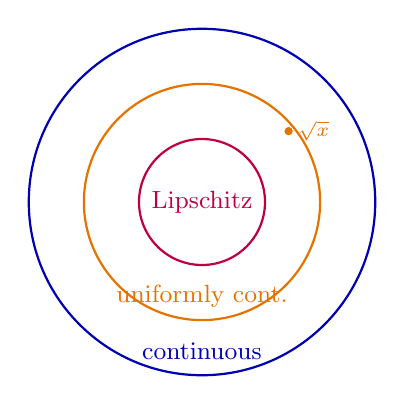
\begin{tikzpicture}[scale=1.0]
  \draw[blue!70!black, thick] (0,0) circle (2.2);
  \node[blue!70!black, font=\small] at (0,-1.9) {continuous};
  \draw[orange!90!black, thick] (0,0) circle (1.5);
  \node[orange!90!black, font=\small] at (0,-1.2) {uniformly cont.};
  \draw[purple, thick] (0,0) circle (0.8);
  \node[purple, font=\small] at (0,0) {Lipschitz};
  \fill[orange!90!black] (1.1,0.9) circle (1.5pt) node[right, font=\scriptsize] {$\sqrt{x}$};
\end{tikzpicture}
\end{center}

% Supplement: Linus Lüchinger/Slides/Slides-03-02.pdf, slide 13
% Was an `aiexercise` labelled ex:ai_continuity_classification. It is Linus's exercise, not
% one invented here, so by the ai*-prefix rule it is a plain `exercise` with a provenance
% comment; only the solution below is authored. His domain for the first row was [0.5,1];
% widened to [0,infty) so that the row separates uniform continuity from Lipschitz, which is
% the distinction \cref{rem:continuity_hierarchy} has just drawn.
\begin{exercise}[Classifying continuity]
\label{ex:continuity_classification}
For each of the following functions, determine whether it is continuous, uniformly continuous,
and/or Lipschitz continuous on the given domain:
\begin{center}
\begin{tabular}{ll}
\textbf{Function} & \textbf{Domain} \\
\hline
$\sqrt{x}$ & $[0,\infty)$ \\
$1/x$ & $(0,1)$ \\
$\sgn(x)$ & $(-1,1)$ \\
$|x|^{3/2}$ & $(-1,1)$
\end{tabular}
\end{center}
\end{exercise}


% --- exercises relocated here from the dissolved sheet 3 ---

% Originally: content/exercise-sheets/week-03.tex, problem 3.1
% Source: exercises/Ex3_Analysis2_eng.pdf

\begin{exercise}[3.1 --- Lipschitz or not]
\label{ex:3.1}
Give an example of:
\begin{enumerate}[label=\textbf{(\alph*)}]
  \item A $\tfrac{1}{2}$-Lipschitz function $f : [0,1) \to [0,1)$ that has no fixed point.
  \item A map $f : \mathbb{R}^2 \to \mathbb{R}^2$ that has no fixed point, but is an isometry,
    i.e.\ $\|f(x) - f(x')\| = \|x - x'\|$ for all $x, x' \in \mathbb{R}^2$.
\end{enumerate}
\end{exercise}

% Originally: content/exercise-sheets/week-03.tex, problem 3.6
% Source: exercises/Ex3_Analysis2_eng.pdf

\begin{exercise}[3.6 --- Multiple choice (uniform continuity)]
\label{ex:3.6}
Select all the statements below that are true.
\begin{enumerate}[label=\textbf{(\alph*)}]
  \item The function $(x,y) \mapsto x+y$ is uniformly continuous in $\mathbb{R}^2$.
  \item The function $(x,y) \mapsto xy$ is uniformly continuous in $\mathbb{R}^2$.
  \item The function $(x,y) \mapsto x+y$ is uniformly continuous in $[0,1]^2$.
  \item The function $(x,y) \mapsto xy$ is uniformly continuous in $[0,1]^2$.
\end{enumerate}
\end{exercise}

\begin{remark}
Corsin's third reason to care about compactness (\cref{sec:why_compactness_matters}) is precisely
that a continuous function on a compact space is uniformly continuous, which settles
\cref{ex:3.6}(c) and (d) at once.
\end{remark}

% Originally: content/exercise-sheets/week-03.tex, problem 3.11
% Source: exercises/Ex3_Analysis2_eng.pdf

\begin{exercise}[3.11 --- (*) Uniform continuity and moduli of continuity]
\label{ex:3.11}
Let $(X,d_X)$ and $(Y,d_Y)$ be metric spaces and let $f : X \to Y$.

A \textbf{modulus of continuity} is a function $\omega : [0,\infty) \to [0,\infty]$ such that
$$\omega(0) = 0, \qquad \omega \text{ is nondecreasing}, \qquad \lim_{t \downarrow 0}\omega(t) = 0.$$
(Here $[0,\infty]$ means we also allow the value $+\infty$.) We say that $f$ \textbf{has modulus
of continuity} $\omega$ if
$$d_Y\big(f(x), f(y)\big) \leq \omega\big(d_X(x,y)\big) \qquad \forall x,y \in X.$$
\begin{enumerate}[label=\textbf{\arabic*.}]
  \item Prove that $f$ is uniformly continuous on $X$ if and only if $f$ has a modulus of
    continuity.
  \item \textit{(Bonus 1)} Assume $X \subset \mathbb{R}$ is an interval with the usual distance
    $d_X(x,y) = |x-y|$. Show that the modulus constructed in (1) can be chosen
    \textbf{subadditive}, i.e.\ $\omega(t_1+t_2) \leq \omega(t_1) + \omega(t_2)$ for all
    $t_1, t_2 \geq 0$.
  \item \textit{(Bonus 2)} Assume $X \subset \mathbb{R}^n$ is \textbf{convex}, meaning: for all
    $x_1, x_2 \in X$ and all $\lambda \in [0,1]$, $(1-\lambda)x_1 + \lambda x_2 \in X$. With
    $d_X(x,y) = \|x-y\|$ (Euclidean distance), show again that the modulus from (1) can be chosen
    subadditive.
\end{enumerate}

\begin{remark}[official]
In general metric spaces a modulus of continuity may have infinite value for finite $t > 0$.
Example: $X = \mathbb{Z}$ with the usual distance, $Y = \mathbb{R}$, $f(n) = n^2$. This $f$ is
uniformly continuous on $\mathbb{Z}$ (because points closer than 1 must be equal), but no finite
$\omega(1)$ can bound $|f(n+1) - f(n)| = 2n+1$ for all $n$. Allowing the value $+\infty$ avoids
this issue, and in many familiar settings (e.g.\ intervals/convex sets in $\mathbb{R}^n$) the
resulting $\omega_f(t)$ is finite for all $t$.
\end{remark}

\textit{Official hints:} \textbf{3.11.1:} define the ``worst oscillation at scale $t$''
$\omega_f(t) := \sup\{d_Y(f(x),f(y)) : d_X(x,y) \leq t\}$. \textbf{3.11.2 / 3.11.3:} if
$d_X(x,y) \leq t_1 + t_2$, choose an intermediate point $z$ on the segment from $x$ to $y$ so
that $d_X(x,z) \leq t_1$ and $d_X(z,y) \leq t_2$, then use the triangle inequality in $Y$.
\end{exercise}

% Originally: the \section{Solutions} of content/week-02.tex and content/week-03.tex

\section{Solutions}
\label{sec:continuity_solutions}

% Transition: Claude Opus 5 (High)
Not every solution in this chapter is collected here. \Cref{ex:distance_to_point_continuous}
(\cpageref{ex:distance_to_point_continuous}) and \cref{ex:evaluation_map_continuous}
(\cpageref{ex:evaluation_map_continuous}) are solved where they appear.

\begin{exercisesolution}[Solution to \cref{ex:2.6}]
% Generator: Claude Opus 5 (High)
\textbf{$d$ is $1$-Lipschitz with respect to $d_2$.} Let $x = (x_1,x_2)$ and $y = (y_1,y_2)$ be
points of $X\times X$. Applying the triangle inequality in $X$ twice,
\[d(x_1,x_2) \ \leq\ d(x_1,y_1) + d(y_1,y_2) + d(y_2,x_2),\]
so $d(x_1,x_2) - d(y_1,y_2) \leq d(x_1,y_1) + d(x_2,y_2) = d_2(x,y)$. Exchanging the roles of
$x$ and $y$ bounds the opposite difference in the same way, hence
\[\big|d(x_1,x_2) - d(y_1,y_2)\big| \ \leq\ d_2(x,y),\]
which is $1$-Lipschitz continuity (\cref{def:lipschitz_continuous}) and therefore continuity
(\cref{rem:continuity_hierarchy}).

\textbf{For $d_1$ and $d_3$: yes, still Lipschitz, but the constant changes.} By
\cref{ex:2.5} part 2 we have $d_2 \leq 2d_1$ and $d_2 \leq \sqrt2\,d_3$, so
\[\big|d(x_1,x_2)-d(y_1,y_2)\big| \leq 2\,d_1(x,y)
  \qquad\text{and}\qquad
  \big|d(x_1,x_2)-d(y_1,y_2)\big| \leq \sqrt2\,d_3(x,y).\]
This is a general principle rather than a computation: \textbf{Lipschitz continuity survives
passage to an equivalent metric}, with the constant multiplied by the comparison factor.
Continuity survives too, being topological, and by \cref{ex:2.5} the three product metrics
induce the same topology.

% Reclassified from ainote to remark: sharpness of the constant is mathematics.
\begin{remark}[The constant $2$ cannot be improved]
The constant $2$ for $d_1$ is sharp, so $d$ is genuinely \emph{not} $1$-Lipschitz with respect
to $d_1$. Take $X = \mathbb{R}$ with $x := (0,0)$ and $y := (-1,1)$. Then $d(x_1,x_2) = 0$ and
$d(y_1,y_2) = 2$, while $d_1(x,y) = \max\{1,1\} = 1$, so the difference equals exactly
$2 = 2\,d_1(x,y)$. This is worth checking, because the problem asks only \emph{whether} $d$ is
Lipschitz for $d_1$ and $d_3$, and it is easy to answer \qt{yes, with the same constant} without
noticing that the constant has in fact changed.
\end{remark}
\end{exercisesolution}

\begin{exercisesolution}[Solution to \cref{ex:2.7}]
% Generator: Claude Opus 5 (High)
All three arguments are short; the point of giving more than one is to see how differently the
same fact reads through the three definitions of \cref{def:continuous}.

\textbf{Topological (\cref{def:continuous}\textbf{(c)}).} This is the shortest, because
preimages compose. Let $W \subseteq Z$ be open. Then
\[(g\circ f)^{-1}(W) = f^{-1}\big(g^{-1}(W)\big),\]
and $g^{-1}(W)$ is open in $Y$ by continuity of $g$, so its preimage under $f$ is open in $X$ by
continuity of $f$. Hence $g\circ f$ is continuous.

\textbf{Sequential (\cref{def:continuous}\textbf{(b)}).} Let $x_n \to x$ in $X$. Continuity of
$f$ gives $f(x_n) \to f(x)$ in $Y$, and continuity of $g$ applied to \emph{that} sequence gives
$g(f(x_n)) \to g(f(x))$ in $Z$.

\textbf{$\varepsilon$--$\delta$ (\cref{def:continuous}\textbf{(a)}).} Fix $x_0 \in X$ and
$\varepsilon > 0$. Continuity of $g$ at $f(x_0)$ supplies $\eta > 0$ such that
$d_Y(f(x_0),y) < \eta$ implies $d_Z\big(g(f(x_0)),g(y)\big) < \varepsilon$. Continuity of $f$ at
$x_0$, applied to \emph{that} $\eta$, supplies $\delta > 0$ such that $d_X(x_0,x) < \delta$
implies $d_Y(f(x_0),f(x)) < \eta$. Chaining the two, $d_X(x_0,x) < \delta$ implies
$d_Z\big((g\circ f)(x_0),(g\circ f)(x)\big) < \varepsilon$.

\begin{remark}[Why the topological proof is the short one]
All three arguments have the same shape, applying the hypothesis for $g$ first and then feeding
the result to $f$. Only the topological version needs no quantifiers at all, because the set
identity $(g\circ f)^{-1} = f^{-1}\circ g^{-1}$ does the bookkeeping the other two proofs carry
out by hand. This is a fair advertisement for \cref{def:continuous}\textbf{(c)}, which can look
like the least intuitive of the three on first meeting: it is the formulation in which
composition is trivial, and that is exactly why general topology takes it as \emph{the}
definition.
\end{remark}
\end{exercisesolution}

\begin{exercisesolution}[Solution to \cref{ex:continuity_classification}]
% Generator: Claude Sonnet 5 (Medium)
\begin{itemize}
  \item $\sqrt{x}$ on $[0,\infty)$: \textbf{uniformly continuous, not Lipschitz.} Uniform
    continuity follows from continuity on $[0,1]$ (compact, \cref{item:uniform_continuity_compact})
    together with $\tfrac12$-Lipschitz behaviour on $[1,\infty)$ (since $|\sqrt x - \sqrt y| \leq
    \tfrac12|x-y|$ there by the mean value theorem, as $|(\sqrt{\cdot})'| = \tfrac{1}{2\sqrt x}
    \leq \tfrac12$ for $x \geq 1$). Not Lipschitz near $0$: for $x_n :=
    1/n^2 \to 0$, $\dfrac{|\sqrt{x_n}-\sqrt0|}{|x_n-0|} = n \to \infty$, so no global $L$ works.
  \item $1/x$ on $(0,1)$: \textbf{continuous, neither uniformly nor Lipschitz continuous.} For
    $x_n := 1/n$, $y_n := 1/(2n)$, $|x_n-y_n| \to 0$ but $|1/x_n - 1/y_n| = n \to \infty$, so no
    uniform $\delta(\varepsilon)$ (and hence no Lipschitz constant) can work near $0$.
  \item $\sgn(x)$ on $(-1,1)$: \textbf{none of the three}, being discontinuous at $0$.
  \item $|x|^{3/2}$ on $(-1,1)$: \textbf{Lipschitz, hence also uniformly continuous and
    continuous.} $|x|^{3/2}$ is $C^1$ on $(-1,1)\setminus\{0\}$ with $\big|\tfrac{d}{dx}|x|^{3/2}\big|
    = \tfrac32|x|^{1/2} \leq \tfrac32$, and the bound extends across $0$ by direct estimation, so
    $L := \tfrac32$ works globally.
\end{itemize}
\end{exercisesolution}

\begin{exercisesolution}[Solution to \cref{ex:3.1}]
% Generator: Claude Opus 5 (High)
Both parts ask for a map with no fixed point, and each defeats one hypothesis of
\cref{thm:banach_fixed_point} while keeping the other, which is exactly what
\cref{rem:banach_hypotheses} predicts must be possible.
\begin{enumerate}[label=\textbf{(\alph*)}]
  \item Take $f(x) := \tfrac{x+1}{2}$. It maps $[0,1)$ into $[\tfrac12,1) \subseteq [0,1)$, and
    $|f(x)-f(y)| = \tfrac12|x-y|$, so it is $\tfrac12$-Lipschitz. A fixed point would satisfy
    $x = \tfrac{x+1}{2}$, i.e.\ $x = 1$, which is not in $[0,1)$. \textbf{What fails is
    completeness:} $[0,1)$ is not a complete metric space, the iterates
    $x_{n+1} = f(x_n)$ march towards the missing endpoint $1$, and \cref{thm:banach_fixed_point}
    does not apply.
  \item Take the translation $f(x) := x + (1,0)$. It is an isometry, since
    $|f(x)-f(x')| = |x-x'|$ exactly, and $f(x) = x$ would force $(1,0) = 0$. \textbf{What
    fails is the strict contraction:} an isometry has Lipschitz constant $L = 1$, not $L < 1$,
    and $\mathbb{R}^2$ is perfectly complete. Together with part \textbf{(a)} this shows neither
    hypothesis of the fixed point theorem can be dropped.
\end{enumerate}
\end{exercisesolution}

\begin{exercisesolution}[Solution to \cref{ex:3.2}]
% Generator: Claude Opus 5 (High)
\textbf{No continuous extension exists for $xy/(x^2+y^2)$.} Suppose $f$ were continuous on
$\mathbb{R}^2$ and agreed with $xy/(x^2+y^2)$ off the origin. Approach the origin along two
different lines:
\[f\!\left(\tfrac1k,\tfrac1k\right) = \frac{1/k^2}{2/k^2} = \frac12,
  \qquad\qquad
  f\!\left(\tfrac1k,0\right) = 0 \quad\text{for every } k.\]
Both sequences tend to $(0,0)$, so continuity would force
$f(0,0) = \tfrac12$ and $f(0,0) = 0$ simultaneously. Hence no such $f$ exists. (This is the same
function, and the same argument, as \cref{ex:partial_derivatives_not_continuous},
where it reappears to show that the existence of both partial derivatives implies nothing.)

\textbf{Exactly one continuous extension exists for $xy/\sqrt{x^2+y^2}$.} Write
$(x,y) = (r\cos\theta, r\sin\theta)$ with $r > 0$. Then
\[g(x,y) = \frac{r^2\cos\theta\sin\theta}{r} = r\cos\theta\sin\theta,
  \qquad\text{so}\qquad |g(x,y)| \leq \frac r2 = \frac{|(x,y)|}{2}.\]
The bound is uniform in $\theta$, so $g(x,y) \to 0$ as $(x,y) \to (0,0)$, and setting
$g(0,0) := 0$ produces a continuous function on all of $\mathbb{R}^2$.

\textit{Uniqueness} is the part worth spelling out, and it needs no computation at all: the value
at the origin is \emph{forced}. Since $(0,0)$ lies in the closure of
$\mathbb{R}^2\setminus\{(0,0)\}$, any two continuous extensions agree on a dense subset of
$\mathbb{R}^2$, and two continuous functions agreeing on a dense set agree everywhere. To see the
latter, take a sequence from the dense set converging to the point in question and apply
\cref{def:continuous}\textbf{(b)} to both. So the extension is unique whenever it exists, which
is also why the first half of the problem had only to exhibit \emph{two} conflicting limits.
\end{exercisesolution}

\begin{exercisesolution}[Solution to \cref{ex:3.6}]
% Generator: Claude Opus 5 (High)
\textbf{(a), (c) and (d) are true; only (b) is false.}

\textbf{(a) True.} Addition is Lipschitz, hence uniformly continuous
(\cref{rem:continuity_hierarchy}):
\[\big|(x+y)-(x'+y')\big| \leq |x-x'| + |y-y'| \leq \sqrt2\,\big|(x,y)-(x',y')\big|,\]
the last step by Cauchy--Schwarz. So $\delta := \varepsilon/\sqrt2$ works everywhere at once.

\textbf{(b) False.} Multiplication is continuous but not uniformly so on the unbounded domain
$\mathbb{R}^2$. Take
\[p_k := \left(k,\ \tfrac1k\right), \qquad q_k := \left(k,\ 0\right).\]
Then $|p_k - q_k| = \tfrac1k \to 0$, while the values are $k \cdot \tfrac1k = 1$ and
$0$, a constant gap of $1$. So no $\delta$ can work for $\varepsilon < 1$. The failure is exactly
the one described in \cref{rem:continuity_vs_uniform_continuity}: the function steepens without
bound as one runs off to infinity, so the local $\delta$ shrinks without a positive floor.

\textbf{(c) and (d) True,} and both for free: $[0,1]^2$ is closed and bounded, hence
\textbf{compact} by \cref{thm:heine_borel}, and a continuous function on a compact metric space
is automatically uniformly continuous by
\cref{prop:compact_implies_uniformly_continuous} (Corsin's third reason to care about
compactness, \cref{item:uniform_continuity_compact}). No estimate is needed for either.

\begin{remark}
The pair \textbf{(b)} versus \textbf{(d)} is the whole lesson: the \emph{same} function $xy$ is
uniformly continuous on $[0,1]^2$ and not on $\mathbb{R}^2$. Uniform continuity is therefore not
a property of a formula but of a formula \emph{together with its domain}, and compactness of the
domain is what removes the room to run off to a bad point.
\end{remark}
\end{exercisesolution}

\begin{exercisesolution}[Solution to \cref{ex:3.11}]
% Generator: Claude Opus 5 (High)
\begin{enumerate}[label=\textbf{\arabic*.}]
  \item \textbf{($\Leftarrow$) A modulus of continuity forces uniform continuity.} Suppose
    $d_Y(f(x),f(y)) \leq \omega(d_X(x,y))$ for all $x,y$, with $\omega$ as in the statement. Let
    $\varepsilon > 0$. Since $\omega(t) \to 0$ as $t \downarrow 0$, there is $\delta > 0$ with
    $\omega(\delta) < \varepsilon$. If $d_X(x,y) < \delta$ then, $\omega$ being nondecreasing,
    \[d_Y\big(f(x),f(y)\big) \leq \omega\big(d_X(x,y)\big) \leq \omega(\delta) < \varepsilon.\]
    The $\delta$ did not depend on $x$ or $y$, which is precisely
    \cref{def:uniformly_continuous}.

    \textbf{($\Rightarrow$) Uniform continuity produces one.} Following the official hint, define
    the \newterm{modulus of continuity of $f$} as its worst oscillation at scale $t$:
    \[\omega_f(t) := \sup\big\{\,d_Y(f(x),f(y))\ :\ x,y \in X,\ d_X(x,y) \leq t\,\big\}
      \ \in\ [0,\infty].\]
    It has all three required properties. $\omega_f(0) = 0$, because $d_X(x,y) \leq 0$ forces
    $x=y$ by definiteness and then $d_Y(f(x),f(y)) = 0$. It is nondecreasing, because enlarging
    $t$ enlarges the set over which the supremum is taken. And $\omega_f(t) \to 0$ as
    $t \downarrow 0$: given $\varepsilon > 0$, uniform continuity supplies $\delta > 0$ with
    $d_X(x,y) < \delta \Rightarrow d_Y(f(x),f(y)) < \varepsilon$, so every $t < \delta$ has
    $\omega_f(t) \leq \varepsilon$. Finally $f$ has modulus $\omega_f$ by construction, since
    $d_Y(f(x),f(y))$ is one of the numbers the supremum defining $\omega_f(d_X(x,y))$ ranges
    over.
  \item \textbf{(Bonus 1) On an interval, $\omega_f$ is already subadditive.} Let
    $t_1,t_2 \geq 0$ and take any $x,y \in X$ with $|x-y| \leq t_1+t_2$. Choose an intermediate
    point $z$ on the segment from $x$ to $y$ as follows: if $|x-y| \leq t_1$ put $z := y$;
    otherwise let $z$ be the point of that segment at distance exactly $t_1$ from $x$, so that
    $|z-y| = |x-y| - t_1 \leq t_2$. Either way $z \in X$, because $X$ is an interval and $z$ lies
    between $x$ and $y$, and $|x-z| \leq t_1$, $|z-y| \leq t_2$. The triangle inequality in $Y$
    now gives
    \[d_Y\big(f(x),f(y)\big) \ \leq\ d_Y\big(f(x),f(z)\big) + d_Y\big(f(z),f(y)\big)
      \ \leq\ \omega_f(t_1) + \omega_f(t_2).\]
    Taking the supremum over all admissible $x,y$ yields
    $\omega_f(t_1+t_2) \leq \omega_f(t_1) + \omega_f(t_2)$.
  \item \textbf{(Bonus 2) Convexity is exactly what the argument needed.} Repeat part 2 verbatim,
    now reading $|x-y|$ as the Euclidean norm on $\mathbb{R}^n$ rather than the absolute value on
    $\mathbb{R}$: the only property of an interval that was used is that the segment from $x$ to
    $y$ lies inside $X$, and that is the definition of convexity. The intermediate point is
    $z := x + \min\{t_1,|x-y|\}\,\frac{y-x}{|y-x|}$ for $x \neq y$, which lies on the segment and
    satisfies the same two estimates.
\end{enumerate}

\begin{remark}[Why the value $+\infty$ has to be allowed]
The official remark accompanying this problem gives the reason, and it is worth restating: on
$X = \mathbb{Z} \subseteq \mathbb{R}$ the map $f(n) := n^2$ is uniformly continuous for the
trivial reason that any two distinct points are at distance at least $1$. Take
$\delta := \tfrac12$, and the implication holds vacuously. Yet
$|f(n+1)-f(n)| = 2n+1$ is unbounded, so $\omega_f(1) = +\infty$. Parts 2 and 3 rule this out by
hypothesis rather than by luck: on a convex set the intermediate-point construction lets a large
displacement be broken into many small ones, so $\omega_f(t) \leq \lceil t/s\rceil\,\omega_f(s)$
is finite as soon as some $\omega_f(s)$ is. A space like $\mathbb{Z}$ has no intermediate points
to subdivide with.
\end{remark}
\end{exercisesolution}

